\documentclass[a4paper,10pt, fleqn]{article}
%\documentclass[a4paper,10pt]{scrartcl}

\usepackage[utf8]{inputenc}
\usepackage{amsmath,amssymb,amstext}
\usepackage{geometry}
\usepackage{fancyhdr}
\usepackage{listings}
\usepackage{color}
\usepackage{array, graphicx}

\begin{document}
\section{Einführung}
\label{sec:einfuhrung-1}


\subsection{Fehlerrechnung}
\label{sec:fehlerrechnung}

Experiment: Kugel fällt durch zwei Lichtschranken

Durchfallene Strecke $x$ im Schwerefeld der Erde bei Anfangsgeschwindigkeit $v_{0} = 0$ ist
$$ x(t) = \frac{1}{2}gt^{2}$$
mit $g$: Fallbeschleunigung, $t$: Zeit

\subsubsection{statistischer Fehler}
\label{sec:statistischer-fehler}
\begin{itemize}
\item Messwert variiert von Messung zu Messung
\item Verteilung der Messwerte entsprechend statistischer Verteilung.
  Im Normalfail eine ``Gauß-Verteilung'' (``Normalverteilung'')
\end{itemize}
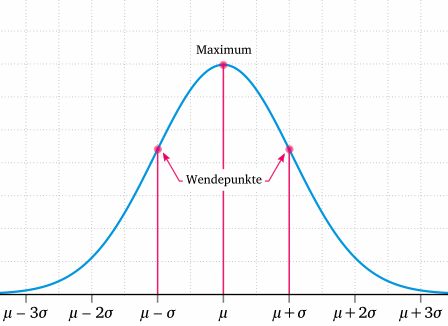
\includegraphics{normalverteilung01.png}
\begin{itemize}
\item $H$: Häufigkeit des Messwertes
\item $x_{wahr} = \mu$
\end{itemize}
$$H(x_{messung}) = \frac{1}{\sqrt{2\pi\sigma^{2}}}e^{-\frac{(x_{messung}-x_{wahr})^{2}}{2\sigma^{2}}}$$
Beste Abschätzung von $x_{wahr}$ aus $N$ Einzelmessungen:
$$\text{arithmetischer Mittelwert:}x_{wahr} \approx \langle  x_{messung} \rangle = \overline{x}_{messung} = \frac{1}{N}\sum_{i=1}^{N}x_{messung, i}$$
\begin{itemize}
\item $\sigma^{2}$: Mittelwert von $(x_{messung} - x_{wahr})^{2}$
\item $\sigma$: mittlerer Fehler einer Einzelmessung
\end{itemize}
Innerhalb des Intervalls $x_{wahr} \pm \sigma$ liegen 68\% der
Messergebnisse, wenn Messwerte gaußverteilt sind.

Abschätzung von $\sigma$:
$$\sigma \approx \sqrt{\langle (x_{messung} - x_{wahr})^{2} \rangle} \approx \sqrt{\frac{1}{N-1}\sum_{i = 1}^{N}(x_{messung, i} - \overline{x}_{messung})^{2}} = \sigma_{M}$$

Fehler des MIttelwerts $\overline{x}_{messung}:$
$$\Delta x = \frac{\sigma_{M}}{\sqrt{N}} = \text{Fehler von } \overline{x}_{messung}$$
$\Rightarrow$ Messergebnis: $\overline{x} \pm \Delta x$

\subsubsection{Systematischer Fehler}
\label{sec:syst-fehl}

Verfälschung des Messergebnisses durch Messmethode oder Messgerät, die
für jede Einzelmessung gleich ist.

\subsubsection{Auswertung Versuch}
\label{sec:auswertung-versuch}

\begin{table}[h]
  \centering
  \begin{tabular}{l | l}
    $t$, $L_{1}$ & $t$, $L_{2}$ \\
    \hline
    0.191s & 0.362s \\
    0.191s & 0.371s \\
    0.191s & 0.363s \\
    0.193s & 0.364s \\
  \end{tabular}
  
  \caption{Daten}
\end{table}
Mittelwert für die Zeit $t$ zum Durchfallen der Strecke $L_{2} = 65cm \pm 1mm$
$$\overline{t} = \frac{1}{4}\sum_{i=1}^{4}t_{i} = \frac{73}{200}s = 0.365s$$
$$\sigma_{M} = \sqrt{\frac{1}{3}\sum_{i = 1}^{4}(t_{i} - \overline{t})^{2}} = 4.08 \cdot 10^{-3}s$$
Genaue Angabe der gemessenen Zeit:
$$\overline{t} \pm \frac{\sigma_{M}}{\sqrt{N}} = 0.365s \pm 2.04 \cdot 10^{-3}s$$
Berechnung der Fallbeschleunigung $g$:
$$L_{2} = \frac{1}{2}g\overline{t}^{2}\Rightarrow g = \frac{2L_{2}}{\overline{t}^{2}} = 9.76 \frac{m}{s^{2}}$$
Echter Wert von $g$:
$$g = 9.81 \frac{m}{s^{2}}$$

\subsubsection{Fehlerfortpflanzungsgesetz}
\label{sec:fehl}

Allgemeiner Fall: Ergebnis $x$ hängt von $m$ Messgrößen
$a_{1},\dots, a_{m}$ ab.
$$x=x(a_{1},\dots, a_{m})$$
Was ist der Fehler von $x$, falls die Unsicherheiten
$\Delta a_{1},\dots, \Delta a_{m}$ bekannt sind?
$$ \Delta x = \sqrt{\sum_{i=1}^{m}\left( \frac{\partial x}{\partial a_{i}} \Delta a_{i} \right)^{2}}$$
$\frac{\partial x}{\partial a_{i}}$: partielle Ableitung der Funktion
$x$ nach der Variablen $a_{i}$, owbei alle anderen Variablen als konstant angenommen werden.

Beispiel: Fehler von $g$?
\begin{multline} \nonumber
  g = \frac{2 L}{t^{2}} \Rightarrow \Delta g = \sqrt{\left(
      \frac{\partial g}{\partial L} \Delta L \right)^{2} + \left(
      \frac{\partial g}{\partial t} \Delta t \right)^{2}}
  = \sqrt{\left( \frac{2L}{t^{2}} \frac{\Delta L}{L} \right)^{2} +
    \left( -2 \cdot \frac{2L}{t^{2}} \frac{\Delta t}{t}\right)^{2}} =
  \sqrt{\left( g \frac{\Delta L}{L} \right)^{2} + \left( 2 \cdot g
      \frac{\Delta t}{t}\right)^{2}} \\
  = g\sqrt{\left(\frac{\Delta L}{L} \right)^{2} + \left( 2 \cdot\frac{\Delta t}{t}\right)^{2}} \\
\end{multline}
Beispiel: $\Delta L = 1mm; \Delta t = 2\cdot 10^{-3}s; L=0.65m; t  = \overline{t} = 0.35s; g = 9.76 \frac{m}{s^{2}}$
$$\Rightarrow \Delta g = 0.11 \frac{m}{s^{2}} \Rightarrow g = (9.76 \pm 0.11)\frac{m}{s^{2}}$$

\section{Mechanik}
\label{sec:mechanik}

Lehre von der Bewegung makroskopischer Körper, Gase oder Flüssigkeiten

\subsection{Kinematik}
\label{sec:kinematik}

Beshreibung der Bewegung von Objekten

\subsubsection{Geradlinige Bewegung, Geschwindigkeit, Beschleunigung}
\label{sec:geradl-beweg-geschw}

Vollständige Beschreibung der Bewegung: Angabe des Ortes $x$ (bzgl.
eines Referenzpunktes) als Funktion der Zeit $t$ $\Rightarrow $ Funktion $x(t)$.

\paragraph{Grafische Darstellung}
...

\paragraph{Geschwindigkeit}

\[
  \text{Geschwindigkeit} = v(t) = \lim_{\Delta t \Rightarrow 0} \frac{x(t + \Delta t) - x(t)}{\Delta t}
  = \frac{dx(t)}{dt} = \dot{x}(t) \text{(nur für Ableitungen nach der Zeit)}
\]
Einheit: $[v] = \frac{m}{s} = m\cdot s^{-1}$, $v(t)$ hängt im Allgemeinen von der Zeit $t$ ab.

\paragraph{Beispiel für geradlinige Bewegung}

Bewegung mit konstanter Geschwindigkeit $v_{0}$
$$x(t) = x(t = 0) + v_{0} \cdot t = x_{0} + v_{0} \cdot t; v(t) = v_{0} = const$$

\textit{[Bild von einer Geraden mit Steigung $v_{0}$ und einer Waagrechten bei $v_{0}$]}

\paragraph{Beschleunigung}

Änderung der Geschwindigkeit. Beschleunigung $a(t)$
$$a(t) = \lim_{\Delta t \rightarrow 0}\frac{v(t + \Delta t) - v(t)}{\Delta t} = \frac{dv(t)}{dt} = \dot{v}(t) = \frac{d^{2}x(t)}{dx^{2}} = \ddot{x}(t)$$
Einheit $[a] = m\cdot s^{-2} = \frac{m}{s^{2}}$ \\
Anmerkung:
\begin{itemize}
\item Jede Änderung der Geschwindigkeit $v$ ist eine Beschleunigung,
  auch wenn $v$ kleiner wird (Abbremsung ist Beschleunigung mit
  negativem Vorzeichen)
\item Bei gleichföriger Bewegung ($v$ = $v_{0}$ = const) ist $a = 0$.

\textit{Einschub: Differenzial und Integralrechnung}
\end{itemize}
\end{document}
%%% Local Variables:
%%% mode: latex
%%% TeX-master: t
%%% End:
